\section{Beantwortung der Aufgaben des Labors zu EMG-Signalen}

\subsection{Aufgabe 1: Darstellung des Messsystems}
Das in Abbildung \ref{fig:blockschlaltbild_lab3} dargestellte Blockschaltbild veranschaulicht den
Aufbau des Messsystems zur Erfassung und Analyse von EMG-Signalen im Rahmen der Laboreinheit.
Die verwendeten Komponenten sind in Tabelle \ref{tab:verwendete_komponenten} aufgelistet und durchnummeriert.
\begin{figure}[h]
    \centering
    \includegraphics[width=1\textwidth]{figures/Blockschaltbild_lab3.png}
    \caption{Blockschaltbild des Messsystems}
    \label{fig:blockschlaltbild_lab3}
\end{figure}
\begin{table}[ht]
  \centering
  \begin{tabularx}{\textwidth}{X c X}
    \hline
    Komponente & Nummer & Verwendung \\
    \hline
    Sparkfun RedBoard & 1 &
      Erfassung der Sensordaten und Übertragung an den Computer \\
    EMG Sensor & 2 &
      Messung der elektrischen Signale des Muskels \\
    Arduino IDE 1.8.19 & 3 &
      Programmierung des Arduino Mikrocontrollers \\
    Python 3.9 & 4 &
      Verarbeitung, Aufzeichnung und Visualisierung der Sensordaten \\
    12 Bit ADC & 5 &
      Wandlung der analogen Sensordaten in digitale Werte \\
    USB A to B Kabel & 6 &
      Verbindung des Arduino mit dem Computer \\
    3 Jumper Kabel & 7 &
      Verbindung des EMG-Sensors mit dem Arduino \\
    Elektroden & 8 &
      Ableitung der elektrischen Signale des Bizeps Brachii \\
    \hline
  \end{tabularx}
  \caption[Verwendete Komponenten und Software]{Die im Rahmen der Laboreinheit verwendeten Komponenten und Software}
  \label{tab:verwendete_komponenten}
\end{table}

Zwischen dem Arduino und dem EMG-Sensor über das Qwicc Kabel wird das I2C (Inter-Integrated Circuit) Kommunikationsprotokoll verwendet. I2C ist ein serielles Kommunikationsprotokoll, das es ermöglicht,
Daten zwischen mehreren integrierten Schaltkreisen (ICs) über nur zwei Leitungen zu übertragen: eine für die Daten (SDA) und eine für den Takt (SCL).
Der Arduino empfängt die Daten über die I2C-Leitungen, verarbeitet sie und leitet sie anschließend an den Computer zur weiteren Analyse und Visualisierung weiter.


\subsection{Aufgabe 2: MVC Durchführung}

\subsection{Aufgabe 3: Darstellung der Ergebnisse aus Aufgabe 2}

\subsection{Aufgabe 4: Aufbau des MVC-Versuchsaufbaus}
Wie in Abbildung \ref{fig:measuring_electrodes} und \ref{fig:GND_electrode_c7} dargestellt, besteht der 
MVC-Versuchsaufbau aus mehreren Komponenten. Am Probanden wurden drei Elektroden angebracht, vergleichbar 
zu jenen, die bereits im Lab~2 verwendet wurden. Zwei Messelektroden wurden auf dem Bauch des Musculus 
biceps brachii platziert, wobei eine Elektrode etwa zwei Zentimeter distal in Richtung der Sehne angebracht 
wurde \ref{fig:measuring_electrodes}. Eine Referenz- bzw. Groundelektrode wurde auf dem Dornfortsatz 
des siebten Halswirbels (C7) positioniert \ref{fig:GND_electrode_c7}. Diese Platzierung wurde gewählt,
um Störungen und bewegungsbedingte Artefakte möglichst gering zu halten.
\begin{figure}[h]
    \centering
    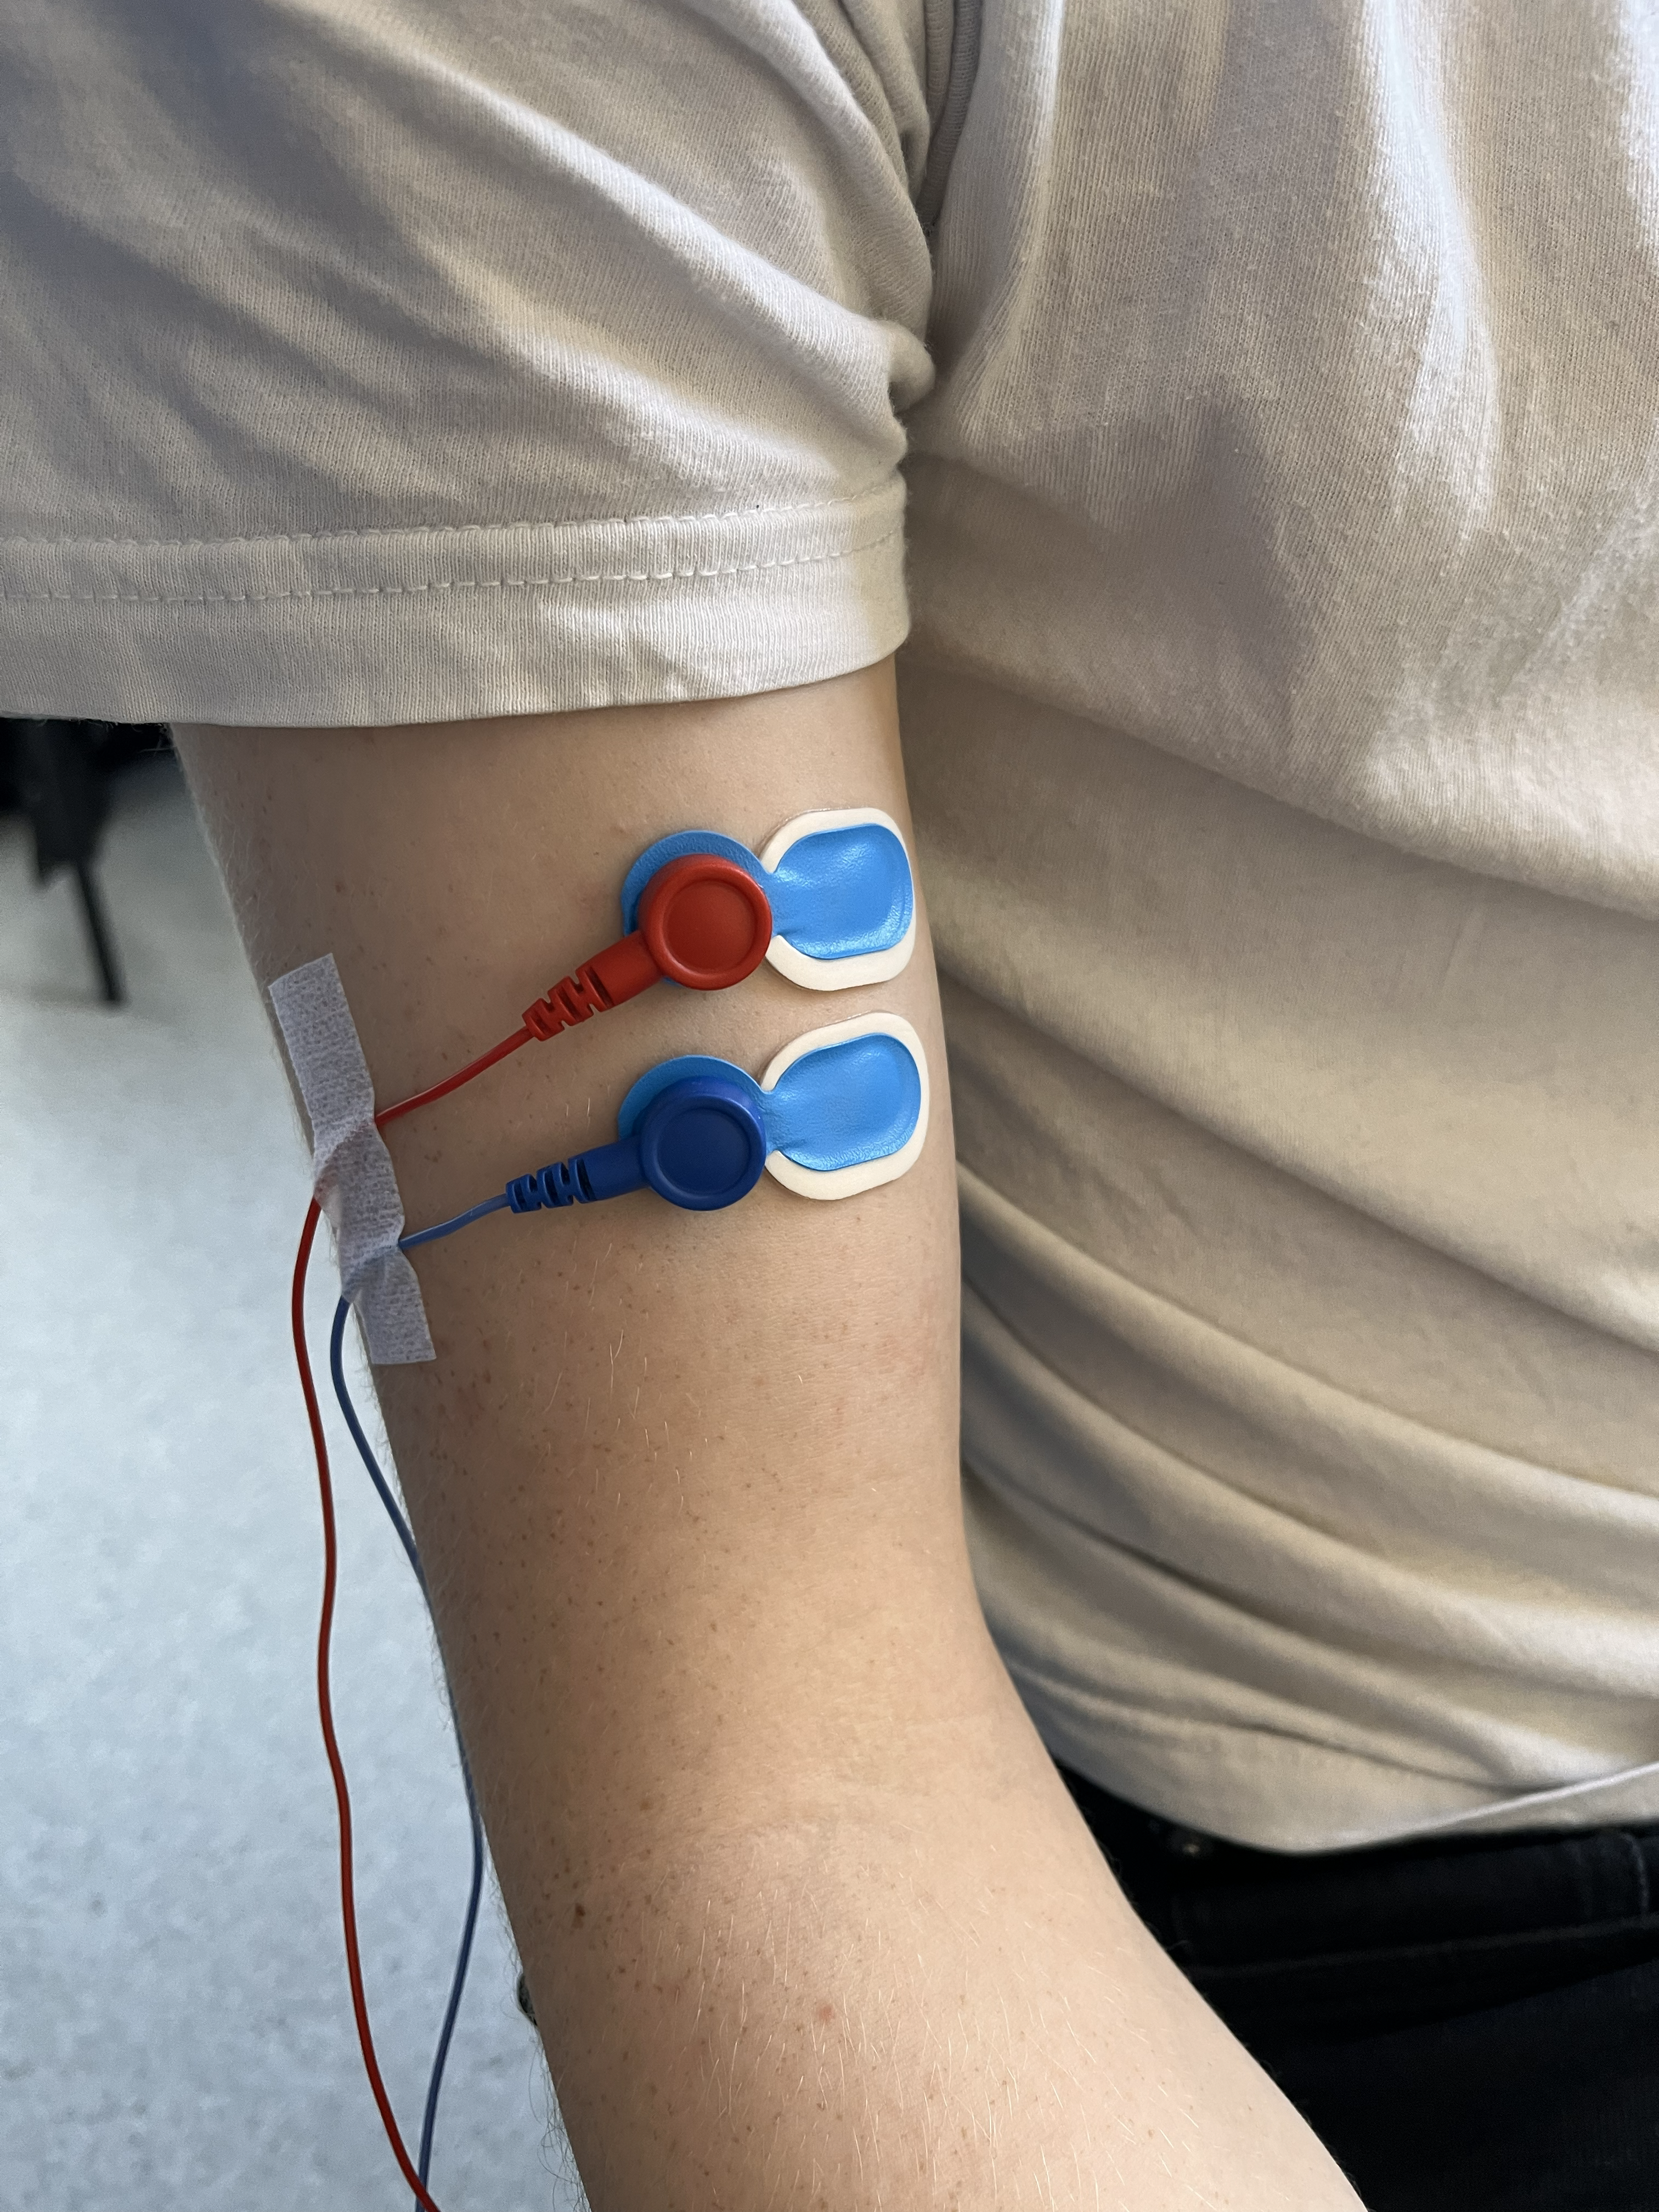
\includegraphics[width=0.3\textwidth]{figures/measuring_electrodes.png}
    \caption{Platzierung der Messelektroden für den MVC-Versuch}
    \label{fig:measuring_electrodes}
\end{figure}
\begin{figure}[h]
    \centering
    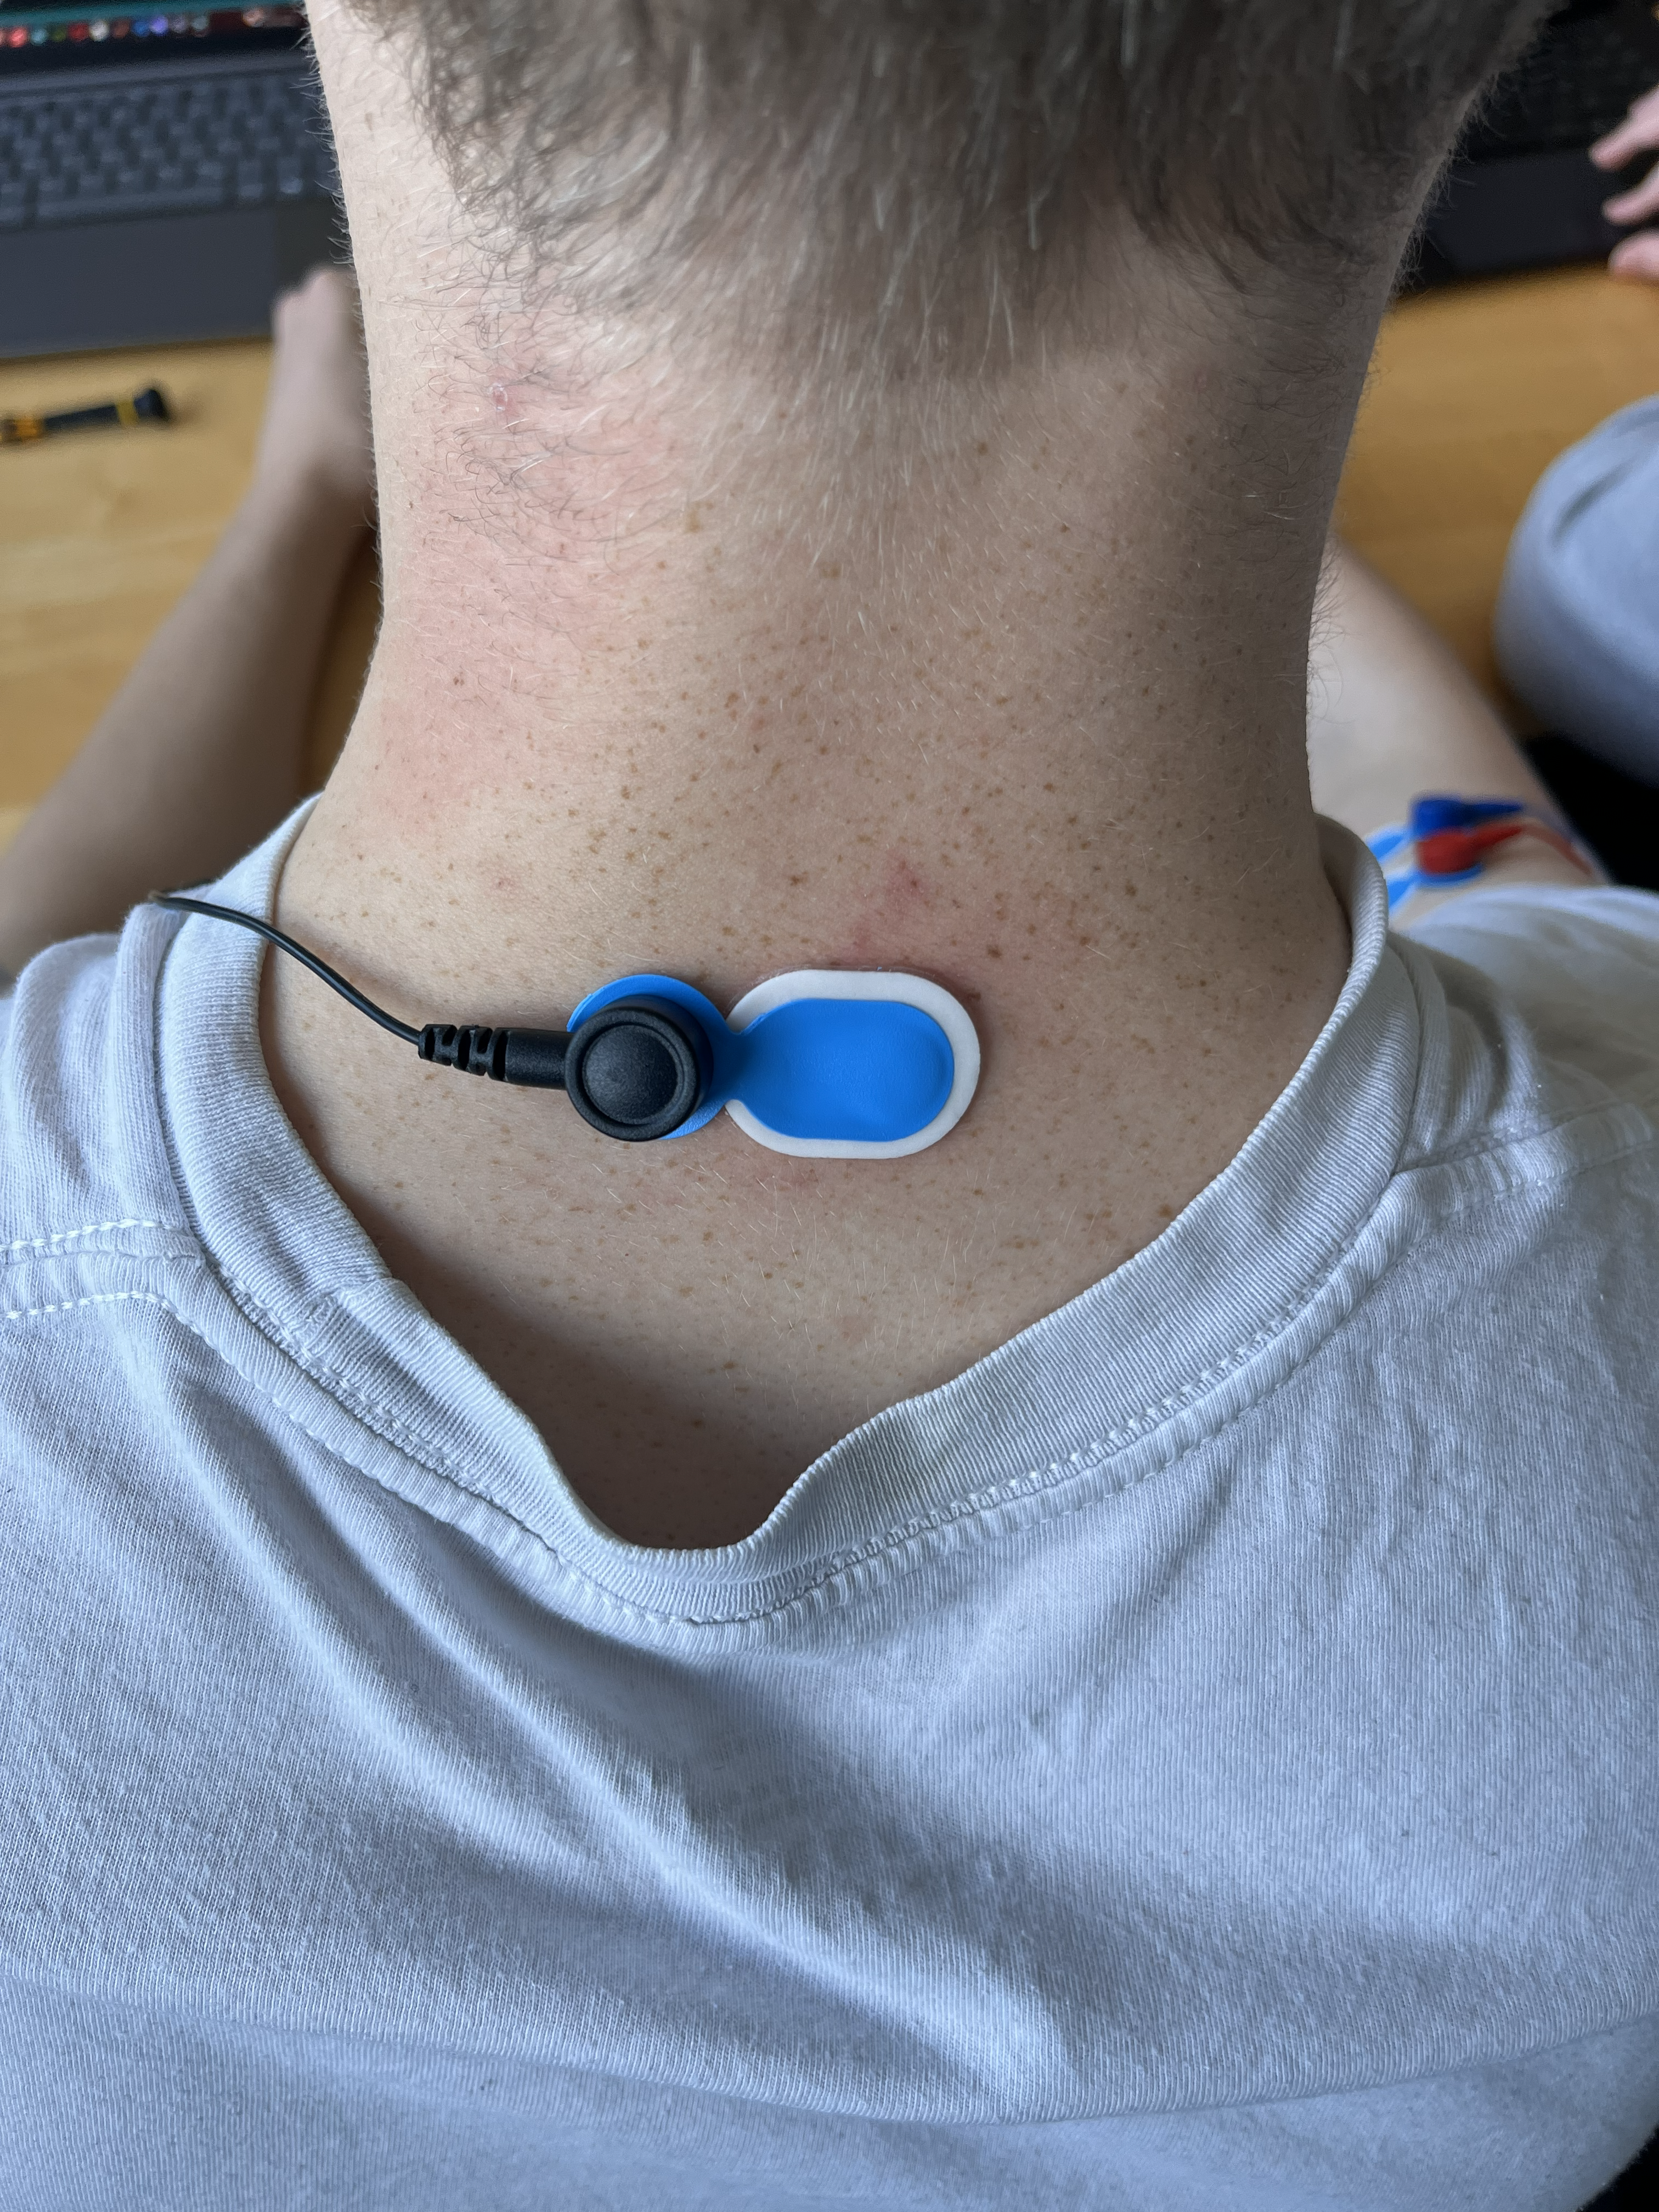
\includegraphics[width=0.3\textwidth]{figures/GND_electrode_c7.png}
    \caption{Platzierung der GND-Elektrode auf dem C7-Wirbel}
    \label{fig:GND_electrode_c7}
\end{figure}
Wie in Abbildung \ref{fig:biceps_tension} zu erkennen ist, sitzt der Proband auf einem Stuhl, wobei der 
Unterarm auf dem Oberschenkel aufliegt. Dadurch stellt sich mit minimaler Bewegung ein etwa 90°-Winkel 
zwischen Ober- und Unterarm ein. Das Handgelenk liegt an der Unterkante des Tisches an. Zur Bestimmung der 
maximalen willkürlichen Kontraktion wird der Proband angewiesen, mit maximaler Kraft zu versuchen, den 
Tisch anzuheben. Gleichzeitig sitzt eine weitere Person auf dem Tisch, um sicherzustellen, dass dieser 
unbeweglich bleibt und keine sichtbare Bewegung stattfinden kann.
\begin{figure}[h]
    \centering
    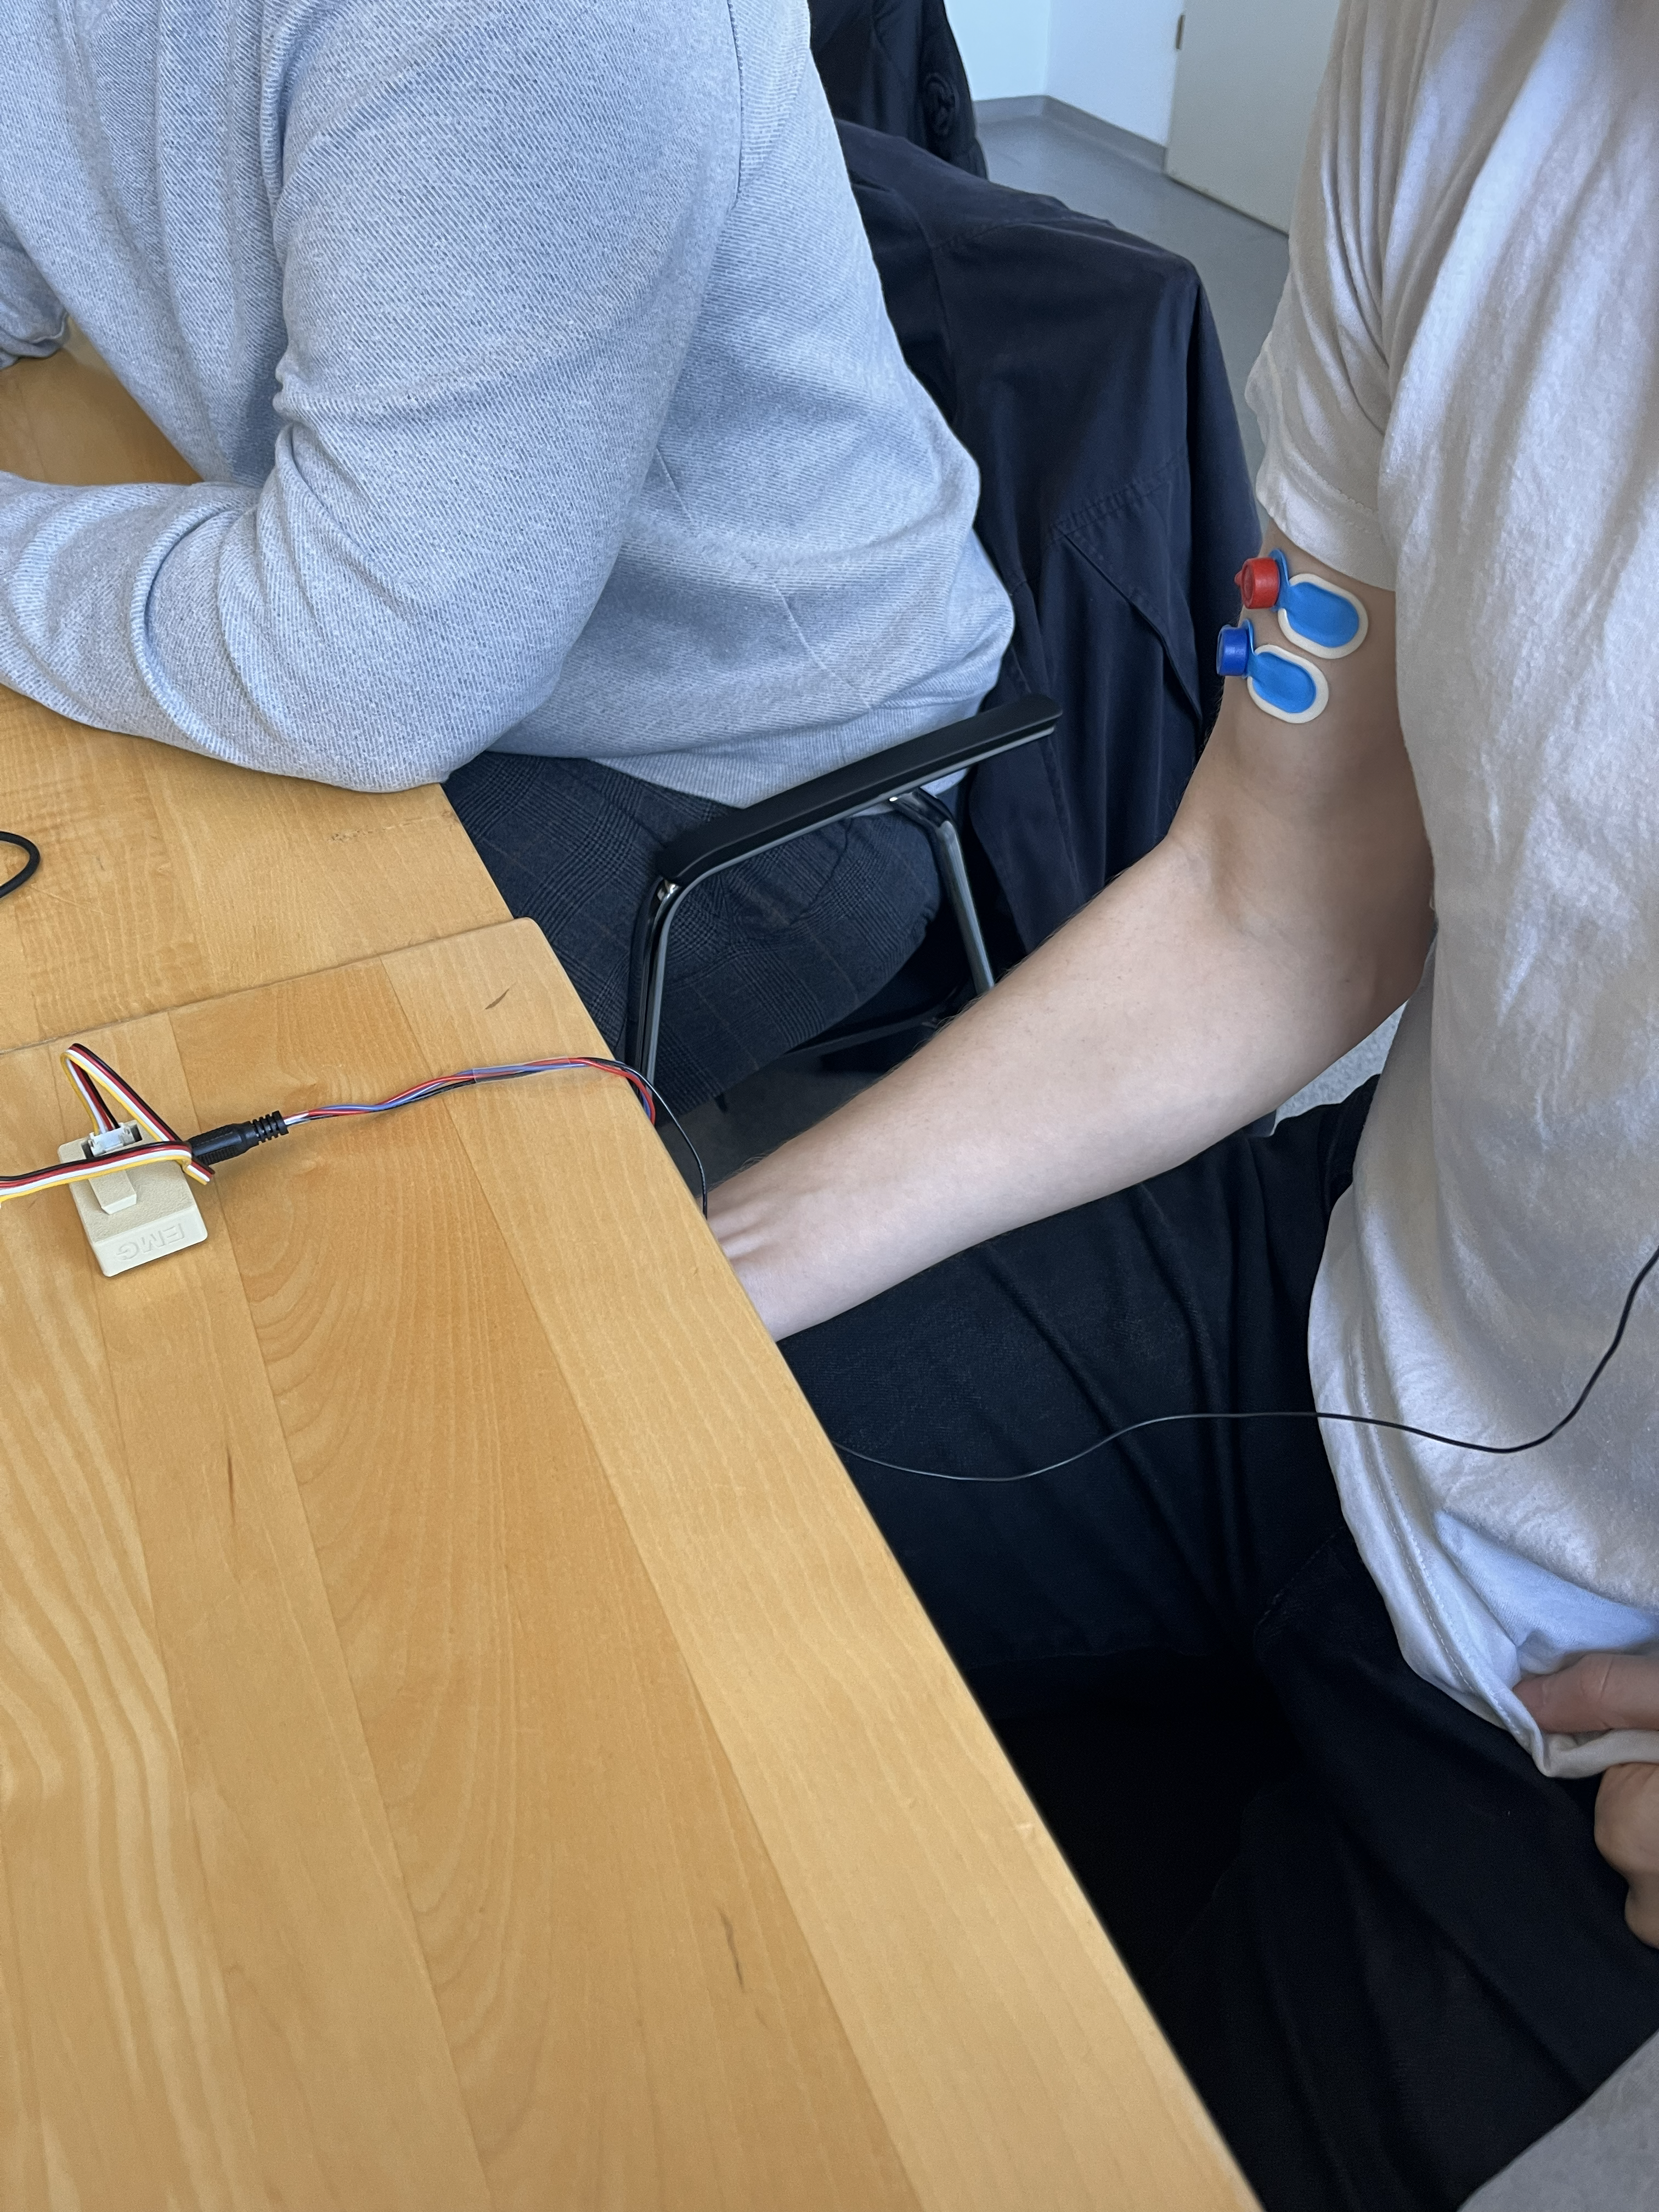
\includegraphics[width=0.4\textwidth]{figures/biceps_tension.png}
    \caption{Angespannter Zustand des Bizeps während des MVC-Versuchs}
    \label{fig:biceps_tension}
\end{figure}
Durch diesen Versuchsaufbau wird eine isometrische Kontraktion des Bizeps brachii ermöglicht, 
bei der der Muskel Kraft entwickelt, ohne sich zu verkürzen. Die gewählte Gelenkstellung begünstigt zudem 
eine nahezu optimale Länge-Spannungs-Relation des Muskels. In Kombination mit der stabilen Körperhaltung 
und dem unbeweglichen Widerstand erlaubt dies eine maximale Rekrutierung motorischer Einheiten und somit 
eine maximale willkürliche Kontraktion.
Die maximale Anspannung wird für acht bis zehn Sekunden gehalten, während die EMG-Daten aufgezeichnet 
werden. Dieser Vorgang wird dreimal wiederholt, wobei zwischen den einzelnen Versuchen eine Pause von etwa
einer Minute eingehalten wird, um muskuläre Ermüdung zu vermeiden. Der MVC-Versuch wurde für alle drei 
Gruppenmitglieder durchgeführt.
Der Bizeps Brachii lässt sich in diesem Versuchsaufbau maximal kontrahieren, da sich um eine isometrische 
Kontraktion handelt und dadurch kein Kraftverlust durch Beschleunigung auftritt.
Zudem bedeutet der 90°-Winkel zwischen Ober- und Unterarm, dass der Bizeps in einer optimalen Länge für
die maximale Kraftentwicklung ist.

\subsection{Aufgabe 5: Experiment 2 -Relative Muskelaktivierung}
@Elias: Kannst du das hier bitte korrekturlesen und ggf. anpassen? Ich hab wenig Ahnung wie unser Plot aussieht haha
\newline
Zur Bestimmung der maximalen willkürlichen Kontraktion (MVC) wurden die drei MVC-Messungen zunächst 
gemittelt. Mithilfe der Einhüllenden der EMG-Signale konnten die Aktivierungsphasen eindeutig identifiziert 
und zeitlich abgegrenzt werden. Innerhalb dieser Intervalle wurde der Mittelwert der Muskelaktivierung 
berechnet und anschließend über alle drei Durchläufe gemittelt. Der so ermittelte Wert stellt die 
individuelle maximale willkürliche Kontraktion dar und dient im Folgenden als Referenzgröße.
Die Auswertung der Belastungsversuche zeigt eine deutlich geringere Muskelaktivierung im 
Vergleich zur MVC. Die gemessene Aktivität liegt erwartungsgemäß bei einem Bruchteil der maximalen 
willkürlichen Kontraktion und skaliert proportional mit der aufgebrachten Last. Dies bestätigt, dass 
für das Halten submaximaler Gewichte nur ein Teil der verfügbaren motorischen Einheiten rekrutiert 
werden muss.

\subsection{Aufgabe 6: Experiment 3 - Ermüdung}
Hier fehlt nur ein Plot und eine schnelle Einordnung, es ist kein weiterer Text gefragt.
\newline
vllt reicht das hier ja schon:
\newline
Im Ermüdungsexperiment bleibt die relative Muskelaktivität zunächst auf einem nahezu 
konstanten Niveau. Im weiteren Verlauf ist jedoch eine leichte Zunahme der EMG-Amplitude zu beobachten. 
Dieses Verhalten ist typisch für ermüdende Muskeln und lässt sich durch eine zusätzliche Rekrutierung 
motorischer Einheiten sowie eine erhöhte neuronale Ansteuerung kompensieren, um die geforderte Kraft 
trotz nachlassender Muskelleistungsfähigkeit aufrechtzuerhalten.
Insgesamt entsprechen die Ergebnisse den physiologischen Erwartungen und bestätigen die Eignung der 
MVC-Normierung zur vergleichbaren Bewertung der Muskelaktivität zwischen unterschiedlichen 
Versuchsbedingungen.

\subsection{Aufgabe 7: Darstellung des Leistungsspektrums}
Wie in Abbildung \ref{fig:beispielbild} dargestellt, zeigt das Leistungsspektrum des EMG-Signals eine 
deutliche Konzentration der spektralen Anteile im niedrigen Frequenzbereich.
\begin{figure}[h]
    \centering
    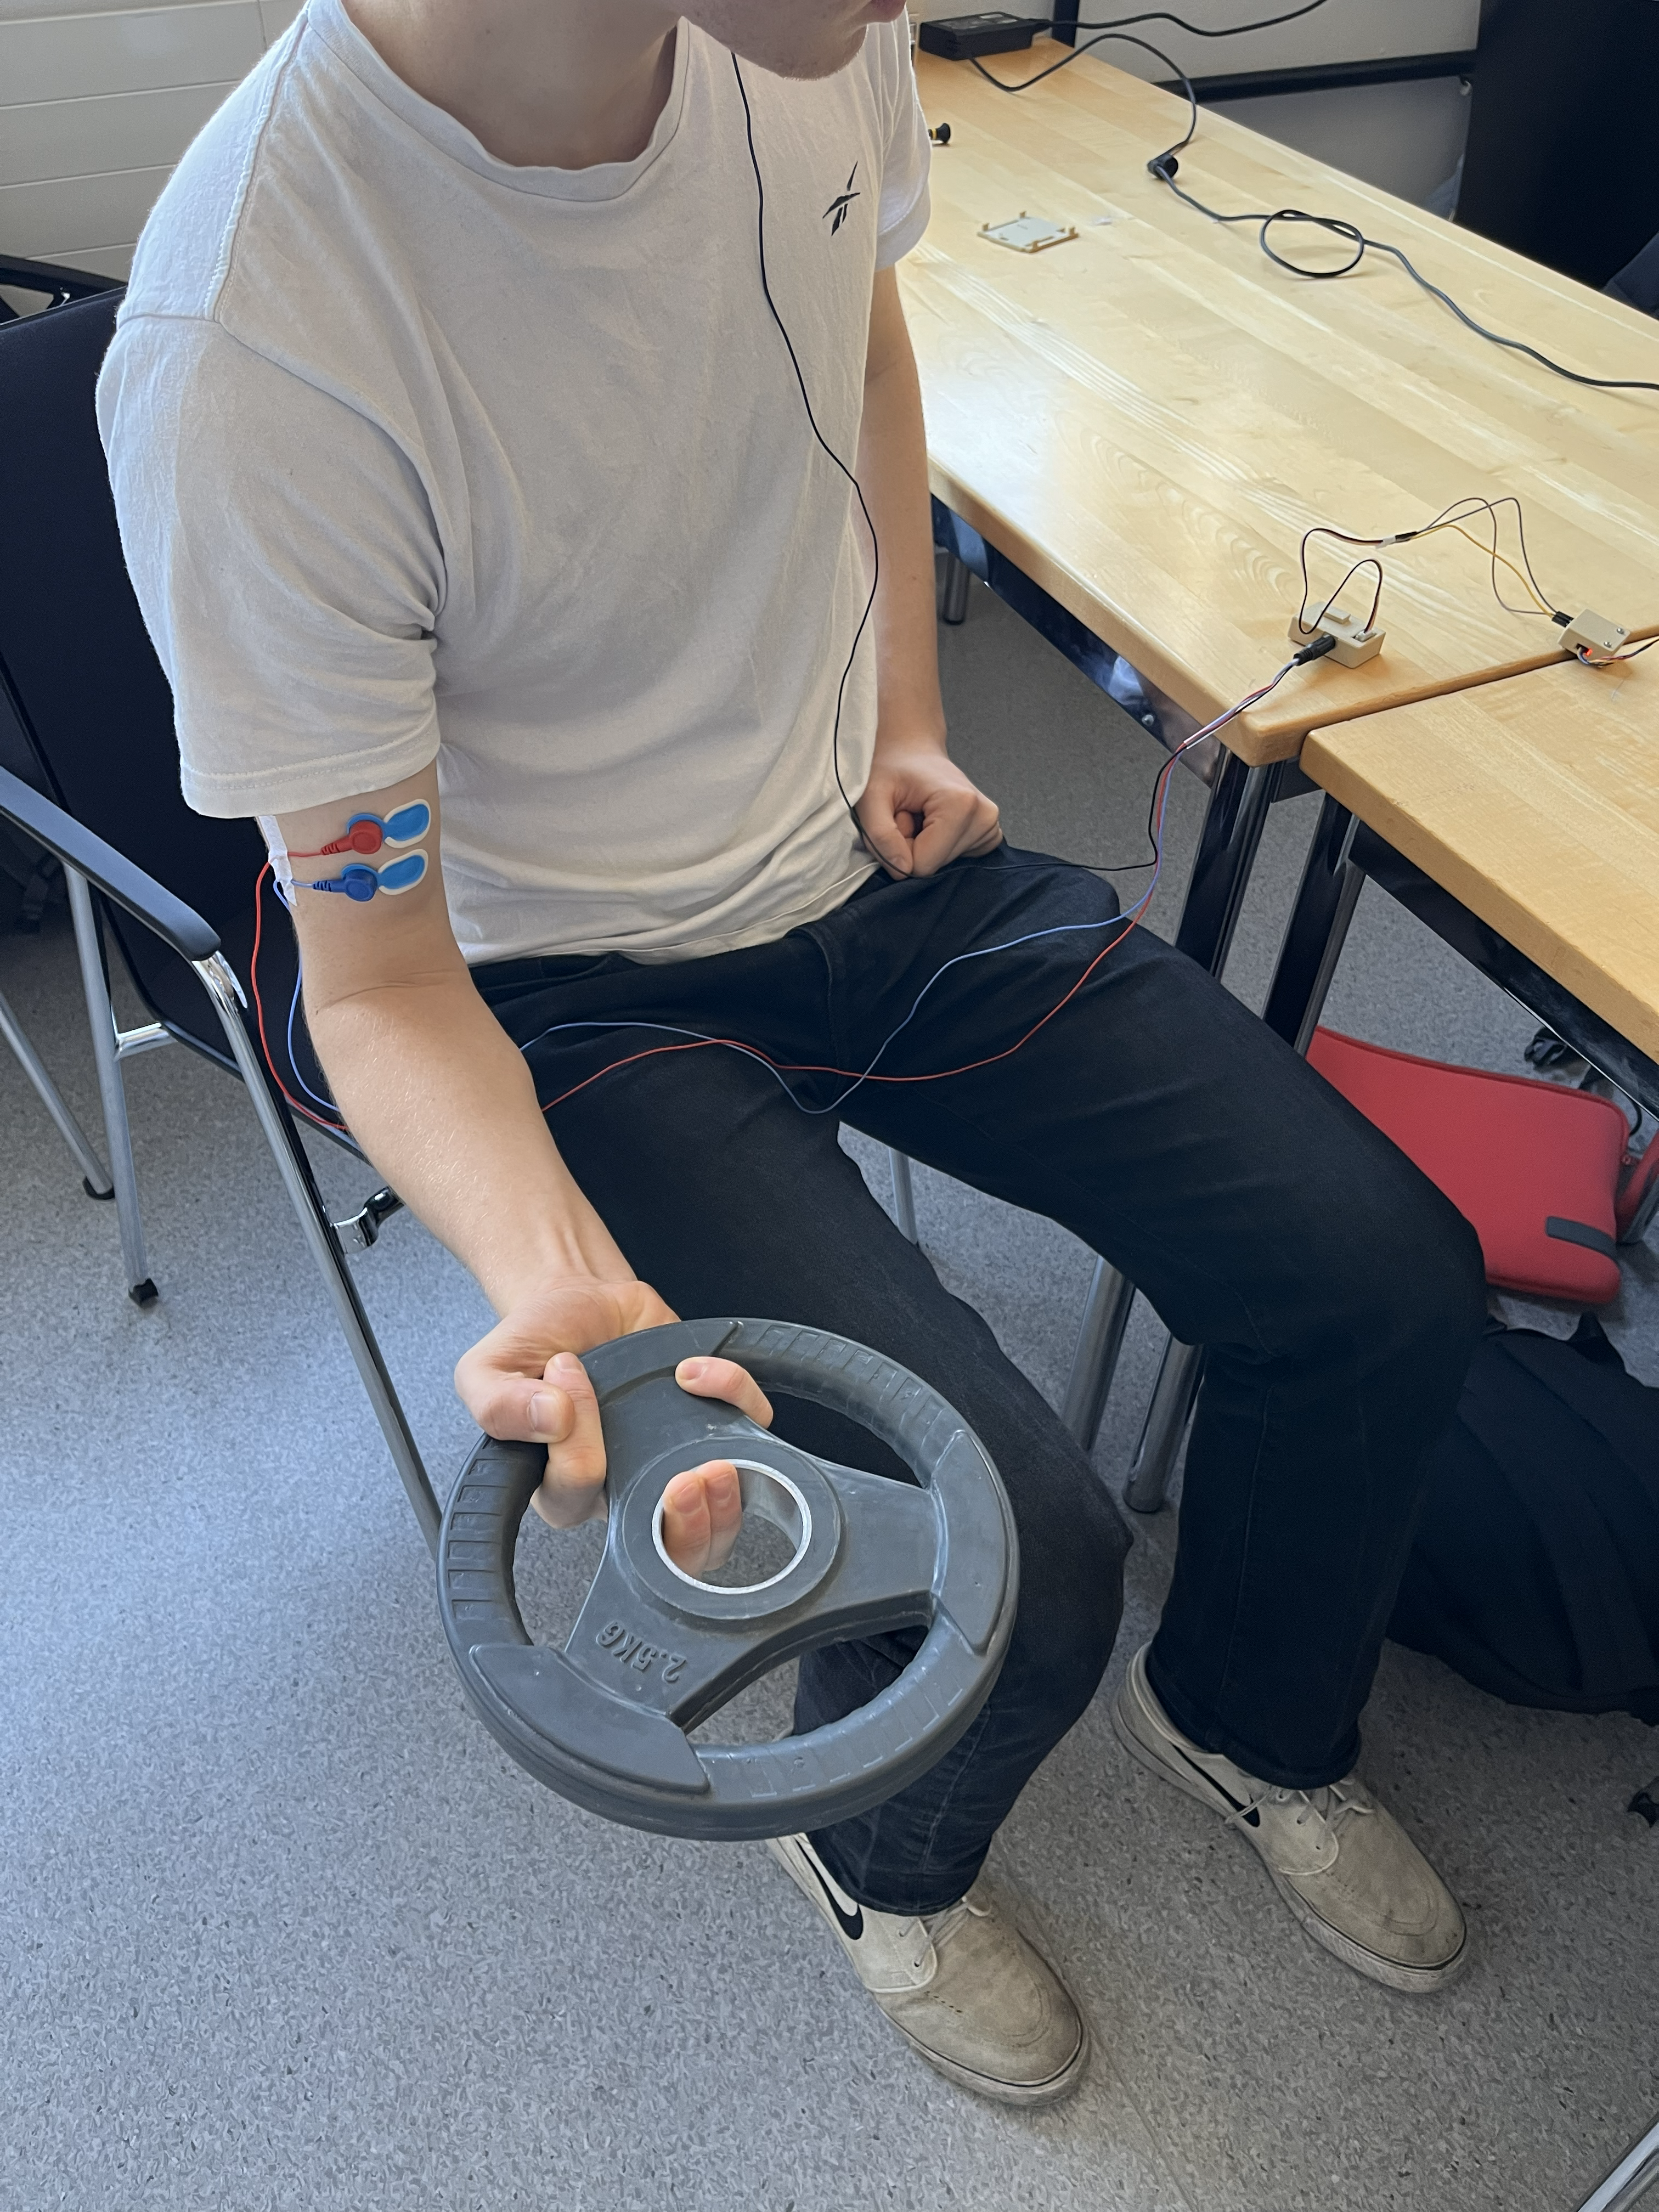
\includegraphics[width=0.3\textwidth]{figures/weight1.png}
    \caption{Beispielbild}
    \label{fig:beispielbild}
\end{figure}
Dieses Spektralverhalten ist charakteristisch für EMG-Signale während isometrischer Kontraktionen und 
statischer Haltearbeit. Entsprechend liegt auch die Medianfrequenz des Leistungsspektrums im unteren 
Frequenzbereich. Dies weist auf eine dominante Aktivierung von Typ-I-Muskelfasern (Slow-Twitch-Fasern) 
hin, die aufgrund ihrer geringen Kontraktionsgeschwindigkeit und hohen Ermüdungsresistenz besonders für 
ausdauernde Belastungen geeignet sind.
Da das statische Halten eines Gewichts über einen längeren Zeitraum eine Ausdauer- und keine 
Schnellkraftbelastung darstellt, ist die niedrige Medianfrequenz physiologisch plausibel. Veränderungen 
der Medianfrequenz im zeitlichen Verlauf können nach Merletti \cite{Merletti1999SENIAM_SignalProcessing} somit als geeigneter Indikator für muskuläre 
Ermüdungsprozesse herangezogen werden, da eine Abnahme der Medianfrequenz typischerweise mit einer 
Reduktion der Muskelfaserleitgeschwindigkeit einhergeht.

\subsection{Aufgabe 8: Medianfrequenz des Leistungsspektrums}